\documentclass[output=paper]{langscibook}
\ChapterDOI{10.5281/zenodo.5483102}

\author{Elena Karagjosova\affiliation{Freie Universität Berlin}}
\title{Mirativity and the Bulgarian evidential system}
\abstract{This paper provides an account of the Bulgarian admirative construction and its place within the Bulgarian evidential system based on (i) new observations on the morphological, temporal, and evidential properties of the admirative, (ii) a critical reexamination of existing approaches to the Bulgarian evidential system, and (iii) insights from a similar mirative construction in Spanish. I argue in particular that admirative sentences are assertions based on evidence of some sort (reportative, inferential, or direct) which are contrasted against the set of beliefs held by the speaker up to the point of receiving the evidence; the speaker's past beliefs entail a proposition that clashes with the assertion, triggering belief revision and resulting in a sense of surprise. I suggest an analysis of the admirative in terms of a mirative operator that captures the evidential, temporal, aspectual, and modal properties of the construction in a compositional fashion. The analysis suggests that although mirativity and evidentiality can be seen as separate semantic categories, the Bulgarian admirative represents a cross-linguistically relevant case of a mirative extension of evidential verbal forms.

\keywords{mirativity, evidentiality, fake past}
}


\begin{document}
\SetupAffiliations{mark style=none}
\maketitle

\section{Introduction}\label{sec:intro}

The \ili{Bulgarian} evidential system is an ongoing topic of discussion both with respect to its interpretation and its morphological buildup. In this paper, I focus on the currently poorly understood admirative construction. The analysis I present is based on largely unacknowledged observations and data involving the morphological structure, the syntactic environment, and the evidential meaning of the admirative.

Thus, it has largely remained unnoticed that the admirative (i) only allows for imperfect past participles which in admiratives receive a present tense interpretation, (ii) does not only encode direct evidence but may also be based on inferential and hearsay evidence, and (iii) is not only used in exclamatives but also in declaratives and is thus not tied to the exclamatory illocutionary force.

Based on these facts, I suggest an analysis of the admirative construction in terms of a semantic operator which captures the evidential, temporal, aspectual, and modal properties of the construction in a compositional fashion, combining insights from \citeposst{Bustamante2013} analysis of the mirative extension of the \ili{Spanish} imperfect and \citeauthor{Smirnova2011a}'s (\citeyear{Smirnova2011a}, \citeyear{Smirnova2011b}, \citeyear{Smirnova2013}) analysis of the \ili{Bulgarian} evidential. According to my analysis, admirative sentences are assertions based on evidence of some type (reportative, inferential, or direct) which are contrasted against the set of beliefs held by the speaker up to the point of receiving the evidence. The speaker's past beliefs entail a proposition which clashes with the assertion, triggering belief revision and resulting in a sense of surprise.
The crucial idea adopted from \citeauthor{Bustamante2013} is related to the role of the tense and aspect morphology: the fact that the past tense morphology in admiratives is interpreted as referring to the present is accounted for by the assumption that tense is displaced and interpreted not within the assertion but under the admirative operator.
The analysis distinguishes further between mirativity as a semantic category and exclamatory force as an illocutionary category and suggests that although mirativity and evidentiality can be seen as separate semantic categories, the \ili{Bulgarian} admirative shows a cross-linguistically relevant case where evidential verbal forms acquire additional mirative meanings.

The paper is organized as follows. \sectref{sec:BG_evid_syst} provides some background on the \ili{Bulgarian} evidential system, the notion of mirativity, and previous work on the \ili{Bulgarian} admirative and outlines the main points of departure for my analysis of the admirative. In \sectref{sec:BG-admirative}, I discuss data showing that the \ili{Bulgarian} admirative differs from other related evidential categories in terms of its temporal, evidential, and modal properties. \sectref{sec:admirative-analysis} presents my account of these properties in terms of their relation to the special morphology of the admirative construction based on \citeauthor{Bustamante2013}'s analysis of the \ili{Spanish} mirative and \sectref{sec:summary-disc} discusses some consequences and residual issues related to the proposal.


   % Section 2


\section{The Bulgarian evidential system and the notion of mirativity}\label{sec:BG_evid_syst}

Traditionally, two different evidential paradigms are distinguished, morphologically and historically \citep[see][]{Andrejcin1944,Aronson1967}
%Some authors take them as part of the verbal mood system, others like \citet{Bojadziev.etal1999} take them to constitute a different system based on the observation that renarrative forms can be combined with imperative forms, as in \textit{Neka pi\v{s}el.} (`Let him write, it is said'). }
related to the present perfect, each encoding different evidential sources: the \textit{renarrative} expressing reportative \REF{report} and the \textit{conclusive} expressing inferential \REF{k:concl} evidence (see, e.g., \citealt{Bojadziev.etal1999,Pasov1999,Nicolova2008}, and \citealt{Jacobson1971}, who was among the first to call these forms evidential):\footnote{``Inferential'' refers both to inference from observable facts and from knowledge. %contra Smirnova who claims that inferential (conclusive) only possible with inference from observable facts
}

\ea\label{report}
\gll Ivan rabotil / rabotel. \\
Ivan work.\textsc{aor.ptcp} {} work.\textsc{ipf.ptcp} \\
\glt `Ivan worked/works, it is said.'
\ex \label{k:concl}
\gll Ivan e rabotil / rabotel. \\
 Ivan is work.\textsc{aor.ptcp} {} work.\textsc{ipf.ptcp}\\
\glt `Ivan has worked, I infer.'
\z

\noindent This view, reflected in \tabref{tab:traditional}, is based on two assumptions: (i) the two evidential paradigms and the present perfect are formally composed of the present tense form of the auxiliary \textit{săm} `be' and a past \textit{l}-participle that may be based on both imperfect and aorist stems, and (ii) the renarrative differs formally from the conclusive and the perfect in terms of auxiliary drop in the 3\textsuperscript{rd} person singular and plural.
In addition to the tense marking of the \textit{l}-participles (aorist or imperfect),\footnote{Note however that some verbs -- 3\textsuperscript{rd} conjugation verbs as well as verbs like \textit{znaja} `know',
% \textit{mladeja} (`look young'),
 \textit{săm} `be' -- only have one past participle, see e.g. \citet{Nicolova2017}.}
%both PAST (not past and present as in Smirnova): minalo svarsheno/ne- dejatelno prichastie; minalo because of the -l!
the participle stems usually encode either perfective or imperfective verbal/lexical aspect (\textit{vid na glagola}).\footnote{See \REF{ex:aorist-imperf-imperf} and \REF{ex:aorist-imperf-perf} respectively. Note that there exist also verbs with a single form that can be both imperfective and perfective (biaspectual verbs; see, e.g., \citealt{MacDonald.Markova2010,Rivero.Slavkov2014}).

\ea\label{ex:aorist-imperf-imperf}
\gll Pisal / pišel săm.\\
write.\textsc{aor.ipfv} {} write.\textsc{ipf.ipfv} am \\
\glt `I have written'\slash`I have been writing'
\ex \label{ex:aorist-imperf-perf}
\gll Napisal / napišel săm. \\
write.\textsc{aor.pfv} {} write.\textsc{ipf.pfv} am \\
\glt `I have finished writing'\slash`I have been finishing writing'
\z}

\begin{table}[h]
\centering
 \begin{tabular}{lllllll}
 \lsptoprule
 \multicolumn{2}{c}{renarrative} & \multicolumn{2}{c}{conclusive} & \multicolumn{2}{c}{present perfect}\\\cmidrule(lr){1-2}\cmidrule(lr){3-4}\cmidrule(lr){5-6}
aorist	    & imperfect	   & aorist  & imperfect & aorist & imperfect\\
 \midrule
pisal săm    & pišel săm	    & pisal săm  & pišel săm & pisal săm & pišel săm\\
pisal $\varnothing$	 & pišel $\varnothing$	 & pisal e	 & pišel e & pisal e & pišel e\\
 \lspbottomrule
 \end{tabular}
 \caption{The traditional Bulgarian evidential forms and the present perfect of the verb \textit{piša} (`write') in \textsc{1sg} and \textsc{3sg}\label{tab:traditional}}
\end{table}

Especially assumption (ii) above has been considered problematic, e.g. in work by \citet{Gerdzikov1984}, \citet{Ivancev1988}, \citet{Levin-Steinmann2004}, or \citet{Sonnenhauser2013}, where the different evidential forms are seen as belonging to one common paradigm (called \textsc{perfect-like complex}; see \citealt{Ivancev1988}), and the usage or omission of the 3\textsuperscript{rd} person auxiliary (called \textsc{auxiliary variation}) as guided by discourse-pragmatic factors such as the coding of the point of view of the narrator vs. some non-narrator (\citealt{Sonnenhauser2013}; see also \citealt{Friedman1981,Lindstedt1994,Fielder99}). Formal semantic work, on the other hand, assumes a single evidential construction called \textsc{perfect of evidentiality} \citep{Izvorski1997} or \textsc{the evidential morpheme/marker} (\citealt{Smirnova2011a,Smirnova2011b}, \citeyear{Smirnova2013}, \citealt{Koev2017}), formally uniquely characterized by a 3\textsuperscript{rd} person auxiliary drop.


As far as the interpretation of the evidential forms is concerned, formal analyses range from their encoding (i) indirect (reportative, inferential) evidence \citep[see][]{Izvorski1997}, (ii) indirect or direct evidence depending on the context (see \citeauthor{Smirnova2013}), and (iii) not encoding evidence at all (see \citealt{Koev2017}). Thus \citeauthor{Koev2017} argues that the evidential forms merely indicate a spatio-temporal distance between the event described by the sentence and the event of the speaker acquiring the evidence for his claim, from which the evidential meaning is pragmatically derived. \citeauthor{Smirnova2013}, on the other hand, assumes that the evidential encodes a temporal relation between the \textsc{evidence acquisition time} (EAT) and the \textsc{speech time} (ST) that, depending on context, is that of precedence (in reportative and inferential contexts) or coincidence (in direct contexts with exclamatory intonation), thus providing a formal account of the compatibility of the evidential forms with the expression of direct evidence.

In the grammatical tradition, uses of evidential forms in direct evidential contexts are dealt with by assuming a further evidential category or paradigm \citep[see][]{Stankov1969} called the \textsc{(ad)mirative}, involving auxiliary drop in the 3\textsuperscript{rd} person and expressing surprise over some suddenly discovered fact or event, see \REF{admir}.\footnote{In addition, a fourth evidential category is sometimes assumed, the \textsc{dubitative}. It involves two further forms of the auxiliary -- present (\textit{săm}) and the past participle (\textit{bil}) -- and auxiliary drop in the 3\textsuperscript{rd} person. It expresses the speaker's doubt with respect to the truth of some renarrated proposition, see, e.g., \citet{Bojadziev.etal1999}, \citet{Pasov1999}. I assume for now that the dubitative is an additional interpretation of the renarrative in accordance with \citet{Bojadziev.etal1999} and do not deal with it in this paper.}

\ea\label{admir}
\gll Ivan rabotel! \\
Ivan work.\textsc{ipf.ptcp} \\
\glt `Ivan works!'
\z

\noindent First noticed by \citet{Weigand1923/1925}, the status of the admirative is subject to continuing debate. While Weigand considers the admirative as a special use of the present perfect, others like \citet{Aleksova2003} and \citet{Kim.Aleksova2003} argue that the admirative is a special, expressive use of the conclusive that indicates a mismatch between what is expected based on inference and the actual state of affairs \citep[see also][]{Besevliev1928,Ivancev1976,Guentcheva1990}. On the other hand, \citet{Andrejcin1938} views the admirative (which he calls ``inopinativus'') as a special use of the renarrative forms serving the expression of facts unexpected for the speaker \citep[see also][]{Nicolova1993,Bojadziev.etal1999,Hauge1999}. The semantics of the admirative is described in \citet{Nicolova2013} more specifically in terms of asserting a state of affairs $p$ and expressing surprise over $p$, where $p$ is discovered immediately before the speech time and the surprise stems from the fact that the speaker's previous knowledge implies not-$p$ rather than $p$ \citep[see also][]{Guentcheva1990}.
Finally, while the evidential source indicated by the admirative is generally assumed to be direct, some authors (e.g. \citealt{Aleksova2001,Kim.Aleksova2003,Simeonova2015})  argue that other evidential sources such as hearsay and inference may also be involved; see \REF{ex:Simeonova}, where the admirative is felicitous in all three evidential contexts:

\eanoraggedright \label{ex:Simeonova}
\textit{Context:} Ivan thought that Stojan did not work. (i) direct evidence: Ivan sees Stojan working.
(ii) inference: Ivan notices that the door to Stojan's study is closed.
(iii) hearsay: Petăr tells Ivan that Stojan is working.
Ivan believes it and exclaims:

\exi{}{\gll Toj rabotel! \\
he work.\textsc{ipf.ptcp}\\ \\
\glt `He works!'\hfill \citep[3; slightly modified]{Simeonova2015}}
\end{exe}


\noindent Based on such evidence, \citet{Simeonova2015} argues in favor of an account of the admirative in terms of mirativity, rather than in terms of evidentiality.

In fact, mirativity as a semantic category encoding the speaker's surprise due to new and unexpected information has been argued to be independent from evidentiality since miratives do not make claims about the source of evidence for the proposition. Rather, this source may be of any kind: direct observation, inference, or hearsay (see, e.g., \citealt{Jacobsen1964,Watters2002}). Mirativity may be expressed by various grammatical forms \citep{DeLancey1997,DeLancey2001,DeLancey2012}, next to other means such as lexicalized adverbials, conventionalized constructions (such as English \textit{(It) turns out (that) S}), and intonation.\footnote{See also \citet[160]{Bustamante2013} on the \ili{Spanish} mirative verb \textit{resultar} `turn out', as well as \citet[290]{TatevosovMaisak1999} on the Tsakhur mirative particle \textit{jī} `it turns out that'.} \citet{Aikhenvald2012} discusses cross-linguistic evidence for a number of grammatical categories, most prominently evidential forms, tense, and aspect that can acquire mirative meanings such as sudden realization, unexpected new information, and surprise. She refers to such extensions of non-mirative grammatical categories towards mirative interpretations in certain contexts as ``mirative strategies''. Differences between evidentials and miratives include the observations that miratives have an assertive force, whereas evidentials typically do not, and that some mirative constructions are restricted with respect to particular tense and/or aspect forms or combinations of tense and aspect forms, whereas evidential constructions do not obey restrictions as to tense and aspect combinations \citep[441]{Aikhenvald2012}.
In spite of these differences, in a number of languages evidential forms such as non-firsthand evidentials or dedicated inferential and reportative evidentials acquire mirative ``overtones'' in certain contexts which can be strengthened by additional means such as particles and interjections (ibid.).

It seems that mirativity and evidentiality are closely intertwined also in the case of the \ili{Bulgarian} admirative. Although the \ili{Bulgarian} admirative does not make claims about a particular evidential source, as indicated by \REF{ex:Simeonova}, it is formally related to the renarrative paradigm in that it involves auxiliary drop, and its tense and aspect morphology is restricted to particular forms and combinations, as will be shown in \sectref{sec:BG-admirative}. Further evidence that will be provided in \sectref{sec:BG-admirative} shows that the \ili{Bulgarian} admirative has assertive force and involves speaker commitment, while the renarrative does not, and differs from the conclusive both in terms of aspectual restrictions and auxiliary behavior. Moreover, I show that the admirative is not only used in exclamative but also in declarative sentences, a property of mirative constructions that has been attested crosslinguistically (see, e.g., \citealt{Bustamante2013}). All these facts suggest that the \ili{Bulgarian} admirative can be seen as a mirative extension of a specific combination of the verbal categories evidentiality, tense, and aspect.

Previous accounts of the admirative do not take these properties into consideration. This concerns first and foremost the aspectual restrictions of the admirative. Although \citet[505]{Smirnova2013} argues that only the ``present tense form of the indirect evidential'' can yield a direct evidential interpretation, she does not account for this property in her analysis.\footnote{Moreover, describing the imperfect \textit{l}-participles in the evidential forms in terms of ``present tense forms'' is not entirely correct, since, as will be shown in \sectref{sec:BG-admirative}, the temporal contribution of the renarrative imperfect participles may, depending on the context, involve reference to the present or the past, due to the well-known syncretism between the participle forms for the present and the imperfect (e.g. \textit{pišel săm}), as well as present perfect and pluperfect (e.g. \textit{bil săm pišel}), and future perfect and past future perfect (e.g. \textit{štjal săm da săm pišel}); see \citet[266]{Andrejcin1944}. This syncretism has been dealt with both in terms of homonymy \citep[e.g.][]{Andrejcin1944} and polysemy or ambiguity \citep[e.g.][]{Demina1959}.} On the contrary, \citeauthor{Smirnova2013} argues that the evidential stems do not encode aspectual difference but carry temporal information only. In addition, there is evidence that the much debated question  of the aspectual properties of the imperfect and the aorist and their relation to the morphological opposition perfective/imperfective (see, e.g., \citealt{Demina1976,Sonnenhauser2006}) is highly relevant for the analysis of the \ili{Bulgarian} evidential system in general and the admirative in particular.

Secondly, earlier accounts rely on the assumption that the admirative is tied to exclamatory mood. Thus, \citet{Aleksova2003}, \citet{Simeonova2015}, and \citet{Sonnenhauser2015} treat all auxiliary-less evidential forms in exclamatives as admiratives.\footnote{See also \citet{Guentcheva2017} who argues that admirative constructions are marked by exclamatory intonation and indicate discrepancy between what is expected and what is observed.} Similarly, \citeauthor{Smirnova2013}'s analysis of the interpretation of evidential forms in direct contexts relies on the assumption that the expression of direct evidence is related to exclamative mood. Instead, I argue with \citet{Bustamante2013} that a distinction must be made between mirativity as a semantic category encoded by various linguistic means (intonation, mirative predicates, verbal morphology) on the one hand and exclamations/exclamatives as illocutionary categories on the other: while both exclamations (declaratives with intonation marking exclamatory force) and exclamatives (special constructions with exclamatory force) can mark the speaker's surprise due to unexpected information,\footnote{\citet{Rett2011} points out that exclamations and mirativity markers both refer to speaker expectations.} there are several properties that distinguish them from mirative constructions in general, such as intonation pattern (which can both be falling and rising with miratives; see more details in \citealt[152--153]{Bustamante2013}), force (declarative for miratives vs. exclamatory for exclamations/exclamatives), and embeddability under certain predicates. Moreover, while miratives indicate a clash with previous beliefs, %Bustamante argues with \citet{Gutierrez-Rexach1996} that
exclamations/exclamatives express a general emotive attitude towards the proposition (surprise, admiration, amazement), which is demonstrated by the acceptability of exclamations in contexts in which the speaker already believes the information expressed but is exclaiming in order to point it out, such as \textit{You overslept again! Which was also to be expected.} \citep[149, 154--155]{Bustamante2013}. In contrast, miratives are not felicitous in contexts in which the speaker already knows or believes the information and are thus
%. \citet[159]{Bustamante2013} takes this evidence as an indication that miratives are
assertions expressing that the speaker has just discovered something unexpected, as will also be shown for the \ili{Bulgarian} admirative. This property indicates that miratives are modalized propositions rather than a kind of speech act \citep[159]{Bustamante2013}.

In addition to disregarding the use of admiratives in declarative sentences, \citeauthor{Smirnova2013}'s account of the use of evidential forms in contexts of direct evidence is further inadequate because it is based on an operator \textsc{excl} which has no illocutionary semantics but is specifically designed to fix the desired temporal relation between the evidence acquisition time EAT and the speech time ST, which in direct evidence contexts is that of coincidence ($\text{EAT}=\text{ST}$) and in indirect evidence contexts one of precedence ($\text{EAT}<\text{ST}$).\footnote{In addition, applying \citeauthor{Smirnova2013}'s analysis to admiratives in declarative sentences would falsely tie the admirative to indirect evidence, as the illocutionary operator \textsc{decl} she defines would lead to an indirect evidence interpretation.} But even genuine illocutionary operators (such as \textsc{e-force} in \citealt[429]{Rett2011}) are unable to account for the relation between the morphological form and the semantic properties of the admirative that will be discussed in \sectref{sec:BG-admirative} and that distinguish the admirative from exclamatory uses of the other two evidential forms, the renarrative and the conclusive.

Finally, considering the \ili{Bulgarian} evidential system as a whole, the assumption of a single evidential morpheme expressing various evidential sources is a simplification that does not account for the actual usage of the \ili{Bulgarian} evidential forms. As will be shown in \sectref{sec:BG-admirative}, it is far from settled that the conclusive involves auxiliary drop. The fact that the admirative is restricted with respect to the form of the \textit{l}-participle militates against such a view as well. In addition, formal analyses like \citet{Izvorski1997} and \citet{Koev2017} are unable to accommodate the admirative since they are not compatible with direct evidence: \citeauthor{Izvorski1997}'s analysis relies exclusively on indirect evidence and \citeauthor{Koev2017}'s analysis on spatio-temporal distance between EAT and the event, which is not true for direct evidence. The auxiliary variation hypothesis is not tenable either once the admirative enters the picture: an explanation in terms of pragmatic effects related to points of view would falsely predict that the auxiliary-less admirative forms are tied to a non-narrator.\largerpage

In the next section, I provide evidence for the properties of the \ili{Bulgarian} admirative discussed above which strongly suggests an analysis in terms of a mirative extension of evidential verbal forms.

\section{The Bulgarian admirative}\label{sec:BG-admirative}\largerpage

The \ili{Bulgarian} admirative differs from renarrative and conclusive evidentials in a number of morphological and semantic properties:

\begin{itemize}
    \item While the admirative (which may, similar to the conclusive, be based on inferential evidence) always involves auxiliary drop, the auxiliary of the conclusive may be omitted under certain conditions (discussed below).
    \item Whereas renarrative and conclusive evidentials both use aorist and imperfect participles, the forms of the admirative are restricted to imperfect participles.
    \item The admirative is not only used in exclamations but also in declarative sentences with declarative illocutionary force.
    \item While the admirative expresses speaker commitment to the underlying proposition, the renarrative is underspecified in this respect.\footnote{I do not exclude though that the renarrative expresses the commitment of the reporter towards the reported proposition; see also Smirnova (\citeyear{Smirnova2011a}, \citeyear{Smirnova2013}).}
    \item Whereas in the case of the admirative the past morphology expresses reference to present events, the temporal interpretation of the renarrative may vary between past and present depending on participle type and context.
    \item Admirative sentences are always related to a clash of beliefs, whereas renarrative and conclusive evidentials (and the present perfect for that matter) used in exclamations may express a wider range of emotive attitudes next to (or beyond) surprise.
\end{itemize}

\subsection{Admiratives based on inferential evidence and conclusives with and without auxiliary}

Formal research on the \ili{Bulgarian} evidential system is based on the assumption that the conclusive involves auxiliary drop and is thus formally indistinguishable from the renarrative and the admirative. While \citet{Izvorski1997} and \citet{Koev2017} adopt a single-morpheme assumption without discussing any data or the possibility of auxiliary variation,\footnote{\citet[3, fn. 2]{Koev2017} mentions that ``the use of evidential forms in inferential contexts is somewhat more restricted than their use in reportative contexts'', possibly due to dialectal variation, however without elaborating on any evidence for this contrast. In fact, no data on this topic can be found in what may be considered the main work on \ili{Bulgarian} dialectology, \citet{Stoykov2002}. \citet{Izvorski1997}, on the other hand, seems to assume that evidential forms that retain the auxilary in the 3\textsuperscript{rd} person are ambiguous between the conclusive and the present perfect.}
\citeauthor{Smirnova2013}'s (\citeyear{Smirnova2011a}, \citeyear{Smirnova2011b}, \citeyear{Smirnova2013}) analysis of the evidential is based on data which partly runs against native speakers' intuitions. Thus, examples like \REF{smirnova:infer-acceptability}, intended to demonstrate the use of the auxiliary-less evidential form in inferential contexts, were rejected by all 11 informants in a small-scale acceptability judgement task in favor of an alternative form (imperfect or aorist participle) containing the auxiliary; see \REF{smirnova:infer-acceptability:alternative1} and \REF{smirnova:infer-acceptability:alternative2}.\footnote{The survey involved 11 native speakers born and living in Sofia, 3 male, 8 female, aged between 20 and 80, 10 of them university graduates, 1 high-school graduate. The survey was designed as a forced-choice task, with 5 alternatives to choose from for the target utterance: the verb in its indicative present form, aorist participle with auxiliary, aorist participle without auxiliary, imperfect participle with and imperfect participle without auxiliary. As a reviewer pointed out to me, the fact that the participants could not choose more than one answer could have obscured cases where the version with the auxiliary was possible but less preferred. Still, the survey shows that the preferred forms are the ones containing the auxiliary.}

\eanoraggedright \textit{Inferential context:} Your late aunt Maria spent the
last months of her life in Paris. No one knows why. After the
funeral, you found a first chapter of an unauthored manuscript about Paris in Maria’s papers. You inferred that Maria was writing a book. When one of the relatives asks you how Maria spent the last months of her life, you say:\label{smirnova:infer-acceptability}

\exi{}{\gll Maria pisala kniga. \\
Maria write.\textsc{aor.ptcp.ipfv} book\\
\glt `Maria was writing a book, [I inferred].' \hfill \citep[497; my glosses]{Smirnova2013}}
\ex \label{smirnova:infer-acceptability:alternative1}
\gll Maria e pisala kniga. \\
Maria is write.\textsc{aor.ptcp.ipfv} book\\
\glt `Maria was writing a book, [I inferred].'
\ex \label{smirnova:infer-acceptability:alternative2}
\gll Maria e pišela kniga. \\
Maria is write.\textsc{ipf.ptcp.ipfv} book\\
\glt ‘Maria was writing a book, [I inferred].’
\z

\noindent For two of the items -- \citet[480, (3) and 498, (35)]{Smirnova2013} -- 6 informants preferred the original auxiliary-less version. Looking closer at the contexts of the examples, however, they seem to be ambiguous between inferential, renarrative, and admirative interpretations. Thus, while \citeauthor{Smirnova2013}'s example (3) describes a situation in which the speaker spontaneously informs her husband of a new surprising fact she just has discovered and thus allows for an admirative interpretation, example (35) draws on evidence from a calendar entry of the person the speaker talks about, which can be interpreted as a second-hand evidential source licensing auxiliary-less renarrative forms.

These observations show not only that the usage of \ili{Bulgarian} evidential forms is highly sensitive to context, but also that evidential forms in inferential contexts are not necessarily auxiliary-less and are at least in those cases formally distinguishable from admiratives based on inferential evidence.\footnote{Of course, one could say that the auxiliary-less forms are the ``real'' evidential forms, whereas the ones retaining the auxiliary are forms of the present perfect with a similar conclusive meaning, as \citet{Izvorski1997} seems to suggest.}

At the same time, it seems that the acceptance of auxiliary-less conclusives may not merely be influenced by context but related to some aspectual properties of the evidential form. Thus it seems that the auxiliary may be omitted when the \textit{l}-participle is based on the aorist form of a perfective verb (or a verb like \textit{săm} `be' which is underspecified with respect to aspectual distinctions), while the temporal interpretation of the form remains the same in both versions:

\eanoraggedright\label{stanalo}
\textit{Context:} Ivan, looking at his watch:

\exi{}{\gll To \minsp{(} e) stanalo veče mnogo kăsno.\\
it {} is become.\textsc{aor.ptcp.pfv} already very late\\
\glt `It has already become very late.'}
\end{exe}

\begin{sloppypar}
\noindent For comparison, the insertion of the auxiliary into an admirative sentence changes the temporal interpretation from present to past and renders the sentence infelicitous in the mirative context:
\end{sloppypar}

% % %     \largerpage[2]

\eanoraggedright
\textit{Inferential mirative context:} Ivan thought that Stojan was not working, but then he notices that the light in Stojan's study is on and exclaims:

\exi{}{\gll Stojan rabotel! / \minsp{\#} Stojan e rabotel!\\
Stojan work.\textsc{ipf.ptcp.ipfv} {} {} Stojan is work.\textsc{ipf.ptcp.ipfv}\\
\glt `Stojan is working!\slash Stojan has been working!'}
\end{exe}

\noindent What seems to distinguish the two versions in \REF{stanalo} is what can be described as the emotional intensity of the utterance which is greater without the auxiliary. This effect is neutralized when the conclusive is used in an exclamation:

\ea \label{djavol}
\gll Ja go viž ti, kakvo \minsp{(} e) namislil starijat djavol!\\
well he.\textsc{acc} look.\textsc{imp} you what {} is plotted.\textsc{aor.ptcp.pfv} old.\textsc{def} devil\\ \hfill \citep[150]{Levin-Steinmann2004} \\
\glt `Look what he has plotted, the old devil!'
\z


%even with verbs underspecified for aspectual differences
%Bre, to tuk imalo mnogo materiali
%Bre, to tuk e imalo mnogo materiali

\noindent In contrast, the auxiliary-less evidential form in \REF{smirnova:infer-acceptability} which is considered problematic by my informants is based on an imperfective aorist participle. This indicates that this aspectual combination may be less acceptable without the auxiliary in non-mirative inferential contexts than an aorist perfective participle.\footnote{See also \citet[33]{Levin-Steinmann2004} who discusses an auxiliary-less ``reduced perfect'' ascertaining the existence of some state and mainly involving the perfective aspect.} Clarifying the morphological status of the conclusive goes, however, beyond the scope of the present study and must be left for future work. For my current purposes, it suffices to conclude that admiratives differ formally from conclusives in terms of both aspectual properties and auxiliary behavior.

%cf. also Levin-Steinmann: Die Existenz eines ״reduzierten“ Perfekts in seiner (zustands-)konstatierenden Funktion erkennt
%neben Popželjazkov (Попжелязков 1962: 85) und Staličarski (Сталичарски 1932)
%auch Koseska-Toszewa in bezug auf zahlreiche bulgarische Dialekte an: ״ ...znane z języka
%literackiego tzw. skrócone perfectum, ma również funkcję k o n sta tu ją c ą ..(1977: 78) [... das
%aus der Literatursprache bekannte sog. verkürzte Perfekt besitzt auch eine konstatierende
%Funktion...]. Das Gesagte konzentriert sich in den betreffenden Dialekten, wie auch in der
%Literatursprache zu beobachten, hauptsächlich auf den vollendeten Aspekt (a.a.O.: 79f).

\subsection{Admiratives and declaratives}\label{sec:decl}

As already pointed out, mirative constructions are not tied to exclamatory illocutionary force crosslinguistically. This applies to the \ili{Bulgarian} admirative as well. As the examples below show, sentences containing admirative forms with auxiliary drop and imperfect past participles with present tense interpretation can be used in declarative sentences with non-exclamative, declarative intonation, where they express commitment to the asserted proposition as well as a clash between the proposition and the speaker's past beliefs.

\ea \label{ex:koslukov}
\gll Ne bjah prava, kogato pisah, če Košlukov ne raboti. %[...].
To se okaza ošte po-lošo -- toj rabotel. \\
\textsc{neg} was right when wrote that Košlukov \textsc{neg} work.\textsc{prs}
 it \textsc{refl} turned.out more worse {} he work.\textsc{ipf.ptcp}\\
\glt `I was not right when I wrote that Košlukov wasn't working. It turned out to be worse -- he obviously \emph{is} working.'
\z

\noindent In \REF{ex:koslukov}, the admirative sentence is semantically embedded under the mirative predicate \textit{okazva se} `it turns out' which already makes the mirative meaning of the admirative sentence salient: the speaker indicates that, prior to the discovery of facts suggesting the opposite, her belief base contained the proposition ``Košlukov is not working''.\footnote{Entire example: \textit{Ne bjah prava, kogato pisah, če programnijat direktor v BNT Emil Košlukov ne raboti, zaštoto godinata veče si teče, a vse ošte njama programna shema. To se okaza ošte po-lošo -- toj rabotel. I kato ne moža da ``izraboti'' dobroto predavane ``Denjat započva s kultura'', kompensira s drugi dve predavanija}.
`I was not right when I wrote that the program director of the \ili{Bulgarian} National Television Emil Košlukov wasn't working, since the year has already begun and yet no program plan exists. It turned out to be worse -- he obviously \emph{is} working. And since he did not manage to ruin the good show ``The day begins with culture'', he did it to two other shows instead.' \hfill (\url{http://e-vestnik.bg/27704/})} Since the admirative sentence asserts that Košlukov is working, it suggests that the speaker's belief base has been revised as a result of receiving some evidence. The evidence which causes the belief clash may be of any kind: reported, inferred, or directly observed. Note that neither the presence nor the form (past aorist) of the mirative predicate \textit{okaza se} have an impact on the mirative interpretation: it does not change if \textit{okaza se} is dropped. A sequence of tenses effect can be excluded here since neither the interpretation nor the acceptability of the sentence change when the predicate of the admirative sentence is set to present tense (\textit{raboti} `works'). A past generic reading can also be excluded, since this reading requires the use of the auxiliary. %it is about particular things he did which
%Ne bjah prava, ce, zastoto (se okaz(v)a ce), toj e rabotel/rabotil HA!

A close example is \REF{ex:misleh} where the admirative is used in a belief revision context similar to the one in \REF{ex:koslukov}. This example stems from \citet[68]{Andrejcin1938} and is used to illustrate what he calls the ``inopinative'' use of the forms of the renarrative for the purpose of expressing facts unexpected to the speaker.

\ea \label{ex:misleh}
\gll Misleh, če e zlato, a to ne bilo.\\
think.\textsc{1sg.ipf} that be.\textsc{3sg.prs} gold, but it \textsc{neg} be.\textsc{ipf/aor.ptcp} \\
%minalo nesvarseno vreme ; this verb does not distinguish between 2 particliple forms
\glt `I thought it was gold, but it isn't.'
\z

\noindent Here, the assertion of the admirative sentence that the object in question is not made of gold is contrasted with an earlier opposite belief of the speaker embedded under the epistemic predicate \textit{mislja} `believe' in the past (imperfect) tense. The evidence that causes the belief change may again be of any sort: direct observation, but also inference or hearsay. Note that the verb \textit{săm} `be' belongs to the rather small group of verbs which do not have different participle forms for the imperfect and the aorist. However, a similar example can be constructed where it can be shown that only the imperfect form is appropriate in such contexts:

\ea \label{ex:misleh2}
\gll Misleh, če raboti, a toj ne rabotel / \minsp{*} rabotil. \\
think.\textsc{1sg.ipf} that work.\textsc{3sg.prs} but he \textsc{neg} work.\textsc{ipf.ptcp} {} {} \textsc{aor.ptcp} \\
\glt `I thought he was working, but he isn't.'
\z

\noindent Moreover, a past tense interpretation is only achieved by putting not only the embedded verb in the present perfect, but also its second occurrence, which requires the use of the auxiliary; see \REF{ex:misleh3}.

\ea \label{ex:misleh3}
\gll Misleh, če e rabotel / rabotil, a toj ne *(e) rabotel / rabotil. \\
think.\textsc{1sg.ipf} that be.\textsc{3sg.prs} work.\textsc{ipf.ptcp} {} \textsc{aor.ptcp}, but he \textsc{neg} \phantom{*(}be.\textsc{3sg.prs} work.\textsc{ipf.ptcp} {} \textsc{aor.ptcp} \\
\glt `I thought he was/has been working, but he was not/has not been working.'
\z

\noindent Here, the sentence suggests that the belief revision has occurred further back in the past and does not have any bearing on the present. In order for a construction to express mirativity, the evidence causing the belief revision must have been acquired recently and have bearing on the present.%\footnote{See also the \textsc{recency restriction} in \citet[459--460]{Rett.Murray2013} saying that ``mirative interpretations are only available relatively recently after the speaker's learning that $p$.'' \citep[464]{Rett.Murray2013}.}
\footnote{See also \citeposst{Rett.Murray2013} \textsc{recency restriction} according to which ``mirative interpretations are only available relatively recently after the speaker's learning that $p$.'' \citep[464]{Rett.Murray2013}.}

%Examples like the ones above are treated by some authors not as admiratives (or renarratives) but in terms of conclusives with auxiliary drop, using them as evidence for the existence of such a phenomenon. Thus, \citet{Levin-Steinmann2004} discusses examples of what she takes to be instances of the conclusive\footnote{Which she defines in terms of a "Wiedergabe einer Schlußfolgerung" (`expression of a conclusion'), \citet[19]{Levin-Steinmann2004}.} with auxiliary drop which on closer examination turn out to be cases of mirativity realized by means of admirative forms in declarative or exclamative contexts involving belief change in view of some recent evidence of some sort (often indicated also by mirative predicates like \textit{izliza \v{c}e} and \textit{okaz(v)a se \v{c}e} `it turns/turned out that'). %(übersetzt ins Deutsche mit "erwies sich"
% One such example is \REF{ex:konspirator} where the speaker suddenly realizes how risky it is to be a conspirator, overwhelmed by the seriousness of the possible consequences of his doings.
%
%%Vapreki preduprezdenieto grazdanskijat istez prodalzi gore-dolu v sastija duh.
%%Izleze, ce nego ne go interesuval zivotat na tova razglezeno ot pari i postove malzinstvo. - das hier ist Renarrativ!!Since no clear commitment and belief change but rather reportative evidence
%%izleze, che nego ne go interesuva /# ne go e interesuval
%
%%Ostanahme obace prijateli. I tova bilo za dobro.
%%this is ambiguo because bilo can be impf or aorist: present or past interpretation
%% okaza se, ce tova e za dobro/e bilo za dobro
%
%%p.19: Mozese da si pozivee oste, no tolkoz i bilo otredeno.
%%Oho, ta ti si stanal vece istinski filosof! this is present perfect which she interprets as admirative
%%Vice versa, cases like ... are categorized as admirative, where however I argue we have a case of conclusive with exclamative intonation, not necessarily expressing belief change. This will become clear when I talk about mirativity.
%
%
%\ea \label{ex:konspirator}
%\gll Kolkoto do polizijata, [...] mo\v{z}e\v{s} da sedi\v{s} spokoen. \v{z}iv njama da me imat [...] Kakva măka bilo da si istinski konspirator! \\
%{As for} {to} police.\textsc{def}, [...] can.\textsc{2p.sg.pres} to sit.\textsc{2p.sg.pres} calm. Alive.\textsc{masc.sg} not to me have.\textsc{3p.pl.pres} [] What misery be.\textsc{ipf/aor.ptcp} to be real conspirator \\ \hfill \citep[36]{Levin-Steinmann2004} \\
%\glt `As for the police, [...] you can be calm. They won't have me alive [...] What a misery it is to be a real conspirator!'
%\z

\subsection{Admiratives and renarratives in exclamations}\label{sec:renarr_admir}\largerpage

As already pointed out in \sectref{sec:BG_evid_syst}, most researchers assume that admirative forms and/or mirative interpretations are only licensed when the forms are used in exclamative sentences. I showed in the previous section that this assumption does not correspond to the linguistic facts. In this section, I argue that it is possible to distinguish between admirative forms having mirative (i.e. clash of beliefs) interpretations, on the one hand, and uses of renarrative forms with renarrative semantics used in exclamations where they indicate surprise or other emotive attitudes, on the other. I pointed earlier at evidence suggesting that mirative constructions differ from exclamations/exclamatives with regard to a number of properties. Thus, exclamatory force is not merely related to surprise in terms of clash of beliefs but covers a wider range of emotive attitudes. Consequently, a renarrative form used in an exclamation or exclamative should be expected to have a greater range of meanings than surprise.
%, contra \citet{Smirnova2013} who argues that an evidential form in reportative contexts with exclamatory intonation automatically gets a mirative interpretation. Besides, this does not explain why only imperfect forms with present tense interpretation are licensed in admiratives as compared to exclamatory renarratives.
%
%Peter rabotel! Tova se ocakvase - only renarrative EXCL interpretation, no admirative
%A speaker can repeat a renarrated sentence with EXCL intonation where the speaker is believig what he has heard
Another difference is that while the admirative forms (imperfect evidential forms with auxiliary drop and present tense interpretation) indicate that the speaker is committed to the proposition expressed, exclamative renarratives do not necessarily express such a commitment. Finally, whereas imperfect renarrative forms in exclamative sentences are ambiguous between present and past interpretation, imperfect admirative forms receive only a present interpretation. Consider \REF{ex:Simeonova-rep} where the context only allows the imperfect participle.

\eanoraggedright\label{ex:Simeonova-rep}
\textit{Context:} Ivan thought that Stojan was not working. (i) direct evidence: Ivan sees Stojan working.
(ii) inference: Ivan notices that the door to Stojan's study is closed.
(iii) hearsay: Petăr tells Ivan that Stojan is working.
Ivan believes it and exclaims:

\exi{}{\gll Toj rabotel / \minsp{*} rabotil! \minsp{\#} Tova ne e vjarno. / \minsp{\#} Tova se očakvaše.\\
%alternatively: Kakva laza!
%alternatively: Tova ne me iznedadva
he work.\textsc{ipf.ptcp} {} {} \textsc{aor.ptcp} {} this \textsc{neg} is true {} {} this \textsc{refl} expected\\
\glt `He is working! This is not true.\slash This was to be expected.'}
\end{exe}


\noindent The temporal interpretation of the form in this context is not past but present. In order to get a past interpretation, it is not only necessary to adjust the context (Petăr tells Ivan that Stojan was/has been working), but also the auxiliary must be used, which changes the admirative into a conclusive (or present perfect) sentence with exclamatory intonation.\footnote{The example would be modified as follows:

\eanoraggedright
\textit{Context:} Ivan thought that Stojan was not working. (i) direct evidence (not possible).
(ii) inference: Ivan notices a pile of newly printed paper on Stojan's desk.
(iii) Petăr tells Ivan that Stojan was working. Ivan believes it and exclaims:

\exi{}{\gll Toj e rabotel / rabotil!\\
he is work.\textsc{ipf.ptcp} {} \textsc{aor.ptcp}\\
\glt `He was/has been working!'}
\end{exe}}

% % %     \largerpage[2]

In addition, the admirative sentence cannot be continued by an utterance like ``This is not true'', which indicates that the speaker is committed to the information expressed, nor by a sentence like ``This was to be expected'', which indicates that the speaker's beliefs prior to receiving the evidence have been revised to accommodate the new information.
Now consider the case of the exclamative use of the renarrative in \REF{ex:renarr-excl}. Here, depending on the tense used in the report, the imperfect participle may refer to a present or past eventuality.\footnote{In this case, the tense forms in the report can be \textit{rabóti} (present tense), \textit{rabóteše} (imperfect), or \textit{rabotí} (aorist).} In addition, the exclamative renarrative may express not only surprise and thus commitment to the content uttered but alternatively disbelief (`This is not true!') or some emotive attitude other than surprise (`This was to be expected').

\eanoraggedright\label{ex:renarr-excl}
\textit{Context:} Petăr tells Ivan that Stojan is/was working.
Ivan exclaims:

\exi{}{\gll Toj rabotel! Kakva iznenada! / Tova ne e vjarno! / Tova se očakvaše!\\
he work.\textsc{ipf.ptcp} what surprise {} this \textsc{neg} is true {} this \textsc{refl} expected\\
\glt `He is/was working! What a surprise!\slash This is not true!\slash This was to be expected!'}
\end{exe}

\noindent Also the aorist participle can be used within an exclamative renarrative, as shown in \REF{ex:renarr-excl-aorist}. Here, however, the aorist participle unambiguously shows that the report on which the evidence is based refers to a past eventuality. Apart from this, the observations from the imperfect participle case hold: the attitude expressed may be surprise (and thus commitment), disbelief, or some other emotive attitude:
%%Why mark as renarrated if S believes information? This shows that expressing commitment or not is not the crucial function of the renarrative, but its function is to signal second-hand information source. To point out claim and express his attitude by means of the excl inton.

\eanoraggedright\label{ex:renarr-excl-aorist}
\textit{Context:} Petăr tells Ivan that Stojan worked (yesterday).
Ivan exclaims:

\exi{}{\gll Toj rabotil! Kakva iznenada! {/} Tova ne e vjarno! {/} Tova se očakvaše!\\
he work.\textsc{aor.ptcp} what surprise {} this \textsc{neg} is true {} this \textsc{refl} expected\\
\glt `He worked! What a surprise!\slash This is not true!\slash This was to be expected!'}
\end{exe}

\noindent The different behavior of the imperfect participle forms in the case of the admirative as compared to the renarrative shows that a simple explanation in terms of a mere ambiguity of forms
%(remember that according to traditional grammar the renarrated forms for the present coincide with the forms of the past imperfect, cf. section \sectref{sec:BG_evid_syst})
does not suffice, and an account of the admirative needs to capture these facts.
%
%\ea (Same context as above)\\
%\gll Toj *rabotil/rabotel! \# No tova ne e vjarno.\\ %No tova vsă\v{s}tnost ne e vjarno; Tova ne me iznenadva. checks mirativity\\
%\textit{he work$_{past.aorist.part}$/work$_{past.imperf.part}$}\\
%\glt `He works (currently)! But this is not true.' % This does not surprise me.'
%\z
%
Furthermore, it was shown in \REF{ex:renarr-excl} and \REF{ex:renarr-excl-aorist} that the speaker may use renarrative forms even though she does not believe the reported information, or when she already believes that the proposition is true.
This contradicts earlier accounts like \citet{Smirnova2013} and \citet{Koev2017}. Thus, \citeauthor{Smirnova2013} argues that her evidential operator \textsc{Ev} has a modal component because \textsc{Ev} is infelicitous in reportative contexts when the speaker knows that the proposition $p$ is true or when the speaker knows that $p$ is false.\footnote{\citeauthor{Smirnova2013} assumes more specifically that in inferential and direct evidential contexts the speaker must be committed to the truth of $p$, where the commitment is weaker than in non-modals.} However, she does not consider renarratives used in exclamatives. Contrary to \citeauthor{Smirnova2013}, \citeauthor{Koev2017} argues that the evidential commits the speaker to $p$, explaining dubitative cases in terms of pragmatic weakening through perspective shift (see \citealt[20--25]{Koev2017}). As shown in the above examples, renarrative forms used in exclamations do not require a perspective shift in order to be interpreted as non-committing, nor are they infelicitous in contexts where the speaker already knows that $p$ is false. Moreover, it can be shown that also in declaratives, the renarrative is felicitous in contexts where $p$ is considered false and where no perspective shift is suggested. Thus, the renarrative can be embedded under the predicate \textit{znaja} `know' with the sole interpretation that the speaker knows of the existence of the claim made by some reporter, either without taking a stance as to the truth of the claim, or in a context in which the speaker knows that the reported proposition is false, as shown by the felicitous continuations of the renarrative sentence in \REF{ex:znam}. If the speaker knows that a reported proposition is true, the renarrative is indeed infelicitous and an indicative form must be used.\largerpage[-1]

\ea\label{ex:znam}
\gll Znaja, če Petăr pušel. No ne znam dali naistina puši. {/} No toj văobšte ne puši.\\
%= I know of this claim/act ASSERT(p)\\ %it does not follow P is smoking right now
know.\textsc{1sg.prs} that Petăr smoke.\textsc{ipf.ptcp} but \textsc{neg} know if really smoke.\textsc{3sg.prs} {} but he {at all} \textsc{neg} smoke.\textsc{3sg.prs}\\
\glt `I know that it is claimed that Petăr smokes/smoked. But I don't know if he really does.\slash But he doesn't smoke at all.'
\z

\noindent Similarly, if the renarrative is embedded under the negation of the predicate \textit{znaja} `know' in its past tense form, the only possible interpretation is that the speaker didn't know about the existence of such a claim made by some reporter. At the same time, the sentence is felicitous when the speaker is ignorant with respect to the truth of $p$ or when she knows that $p$ is false.

\ea
\gll Ne znaeh, če Petăr pušel. Az lično njamam predstava dali puši / e pušil ili ne. / Az lično znam, če ne puši / ne e pušil.\\
%I hadn't heard ASSERT(p) (a speech act, or judgement) before
\textsc{neg} know.\textsc{1sg.aor} that Petăr smoke.\textsc{ipf.ptcp} I personally do.not.have idea if smoke.\textsc{3sg.prs} {} is smoke.\textsc{aor.ptcp} or \textsc{neg} {} I personally know that \textsc{neg} smoke.\textsc{3sg.prs} {} \textsc{neg} is smoke.\textsc{aor.ptcp}\\
\glt `I didn't know that Petăr supposedly smokes/smoked. I personally have no idea if he does/did or not.\slash I personally know that he doesn't/didn't smoke.'
\z

\noindent Renarratives behave the same way in exclamatory sentences: they are felicitous both in contexts in which the speaker believes the reported information and is surprised, as in \REF{ex:lazy-guy} which can be continued by an utterance like ``Can you imagine, this lazy guy!'', and in contexts like \REF{ex:what-a-lie} where the speaker is rather outraged by a claim she knows doesn't correspond to the truth and where the sentence with the renarrative can be continued by an utterance like ``What a lie!''.\largerpage[-2]

\eanoraggedright\label{ex:lazy-guy}\sloppy
 \textit{Context:} A learns from B that Ivan worked the previous day which happens to be a Sunday. A is surprised over this fact ($+$\textsc{belief clash}, \hspace{0pt}$+$\textsc{commitment}) and later tells C:

\exi{}{\gll Ivan rabotil včera! \\
Ivan work.\textsc{aor.ptcp} yesterday\\
\glt `Ivan worked yesterday!'}
\ex\label{ex:what-a-lie}
\textit{Context:} A learns from B that Ivan worked the previous day. A does not believe it because she knows the truth but finds the commitment of the reporter B surprising ($-$\textsc{belief clash}, $-$\textsc{commitment}) and later tells C:

\exi{}{\gll Ivan rabotil včera! \\
Ivan work.\textsc{aor.ptcp} yesterday\\
\glt `Ivan worked yesterday!'}
\end{exe}

\noindent These uses of the \ili{Bulgarian} renarrative evdential form suggest that it merely indicates that the speaker has hearsay evidence for $p$, without committing the speaker to its truth.% (i.e. speaker beliefs are not involved).
\footnote{Additional evidence that needs to be examined is that there is a slight difference in intonation pattern, as also observed in \citet[152--153]{Bustamante2013} for the \ili{Spanish} mirative as compared to \ili{Spanish} exclamations: L or H-L in admiratives, H in exclamations.}

\tabref{properties-admir} summarizes the findings in this section.\footnote{Since auxiliary-less conclusives are difficult to distinguish from inference-based admiratives, I leave the question open whether the former may express reference to the present.}

\begin{table}
\caption{Properties of the admirative by comparison\label{properties-admir}}
\begin{tabular}{ll ccc}
\lsptoprule
& & renarr. & concl. & admir.\\\midrule
\multicolumn{2}{l}{auxilary} & $-$ & $\pm$ & $-$\\
\multicolumn{2}{l}{participle} \\
& \textsc{aor} & $+$ & $+$ & $-$\\
& \textsc{ipf} & $+$ & $+$ & $+$\\
\multicolumn{2}{l}{evidential source} \\
& report & $+$ & $-$ & $+$ \\
& infer. & $-$ & $+$ & $+$ \\
& dir.   & $-$ & $-$ & $+$ \\
\multicolumn{2}{l}{speaker commitment} & $-$ & $+$ & $+$\\
\multicolumn{2}{l}{belief clash} & $-$ & $-$ & $+$\\
\multicolumn{2}{l}{time preference}\\
& present & $+$ & ?   &$+$\\
& past    & $+$ & $+$ &$-$\\
\lspbottomrule
\end{tabular}
\end{table}

\section{The admirative operator}\label{sec:admirative-analysis}\largerpage

%The evidence presented in the previous section leads to the conclusion that the admirative is a category separate from renarrative and conclusive evidentials in contemporary \ili{Bulgarian}. I suggest that the admirative can be viewed as a semantic extension of the renarrative, either already grammaticalized or in the process of grammaticalization (cf. \citet{Iliev2017} who claims that the renarrative is still in the process of grammaticalization): in contexts like \REF{ex:lazy-guy} where the speaker expresses surprise due to a clash between old beliefs and new reportative evidence and commitment to the asserted proposition, the imperfect participle forms of the renarrative acquired a mirative evidential meaning which further expanded to include not only reportative but also inferencial and direct evidential sources.
%%only ipf ptcp since only they can have a present tense interpretation
%%Iliev, admirative: "az naucih i tova me ucudva"
%In other words, part of the renarrative paradigm acquired a specialized mirative interpretation which grammaticalized as a separate, mirative evidential category.
In this section, I account for the properties of the \ili{Bulgarian} admirative discussed in the preceding section in terms of the modal evidential operator $\textsc{admir}(p)$ which captures the following facts:

\begin{enumerate}
\item The proposition $p$ is asserted, the speaker is committed to the truth of $p$.
\item $p$ is based on evidence of some sort (direct, inferential, reportative).
\item $p$ clashes with the speaker's beliefs up to the point of getting the evidence.
\item The asserted eventuality is ongoing at speech time.
%\footnote{ EAT $\subseteq$ ET, which follows from the present tense interpretation of the participle (RT=ST) and the imperfective aspect which is the sem. interpret. of IPF: RT $\subseteq$ ET }
%\item RT $\subseteq$ ET (imperf.) %compare
\item The evidence acquisition time immediately precedes or coincides with the speech time. %EAT $\leq$ ST
\end{enumerate}

%\framebreak
%
%	ET\\
% ///////////////////////// \\
%$______________________$$\rightarrow$ \\
%
%EAT, RT, ST
%

To this end, I adopt \citeposst{Bustamante2013} analysis of a \ili{Spanish} mirative construction that involves past imperfect morphology as in \REF{ex:fumaba}.\footnote{The glosses are as in the original example.} Here, the past imperfect does not have its usual temporal meaning expressing reference to a past eventuality but refers to a present eventuality and expresses that $p$ clashes with the speaker's previous beliefs. In addition, this use of the past imperfect indicates that the speaker is commited to $p$ and is felicitous in both direct and inferential evidential contexts.


\ea\label{ex:fumaba}
\gll Juan fum-aba. \hfill \\
Juan smoke-\textsc{past.ipfv.3sg}\\
\glt `Juan smokes!' \hfill (\ili{Spanish}, \citealt[34]{Bustamante2013})\\
\z

%In a similar way, the pluperfect in Andean \ili{Spanish} (which is a complex verbal form consisting of an auxiliary verb in past imperfect and a participle form of the main verb) has also acquired a mirative use where it expresses
%"surprise about episodic eventualities" and can be used for present and past eventualities (ibid.: 35). Thus the mirative sentence in \REF{ex:pluperfect} can be used in a context in which the speaker thought that Juan didn't smoke at the party, but then sees ashes on his clothes. Crucially, the pluperfect in its mirative use does not display its standard meaning of "a past of the past", but the tense is `fake'.
%
%
%\ea \label{ex:pluperfect}
%\gll Juan hab-ia fumado \hfill (ibid.: 36)\\
%Juan Aux.\textsc{PAST.IMPF.3SG} smoke.\textsc{PTCP}\\
%\glt `Juan smoked!
%\z

\noindent Examples like this are taken to suggest that the mirative use of the past imperfective involves ``a shifting of time reference for the eventuality described in the proposition, leaving the past as `fake'{''}, while the (imperfective) aspect retains its usual interpretation \citep[6]{Bustamante2013}. \citeauthor{Bustamante2013} interprets such cases of `fake' past interpretations of past tense morphology and imperfective aspectual morphology as an example of mirative extension of the imperfect (and pluperfect) tense in \ili{Spanish}.
%
%She develops an analysis of such mirative sentences as modal statements introducing a modal mirative operator that relates the assertion to the beliefs of the speaker up to a point in time at which the speaker obtains evidence incompatible with these beliefs. A central assumption is that the [past]-feature of the tense morphology in these mirative statements is not interpreted as the temporal value of the statement but as the temporal value of the modal base containing the past beliefs of the speaker up to the point of discovering the new evidence.
%
% The analysis also accounts for the role of aspect which in the case of the \ili{Spanish} mirative is required to be imperfective,
%\footnote{Cf. also \citet[43]{DeLancey1997} who describes the role of aspect in Sunvar the following way: “What we see here is the grammaticization of sthe pragmatic tendency toward evidential interpretation of new knowledge marking in perfective contexts, and mirative interpretation in imperfect contexts [...]. This could be predicted, since an event that is perfective is typically past, and therefore no longer “new knowledge.”}
%The main idea in \citet{Bustamante2013} is that the past tense morphology of the \ili{Spanish} mirative is crucial for its mirative meaning.
%: "in the mirative use of the past imperfective there is a shifting of time reference for the eventuality described in the proposition, leaving the past as ‘fake'" (ibid: 5).

In contrast to approaches to fake past morphology such as \citet{Iatridou2000}, \citeauthor{Bustamante2013} does not assign a special semantics to this past tense but assumes a regular meaning in terms of \citet[10]{Kratzer1998}.\footnote{\sib{past}$^{g,c}$ is only defined if $c$ provides an interval $t$ that precedes $t_0$. If defined, then \sib{past}$^{g,c}=t$. This definition corresponds to the neo-Reichenbachean past defined in terms of a relation between reference time and speech time ($\text{RT}<\text{ST}$); see, e.g., \citet{Klein1994}.}
The crucial assumption concerns the locus of interpretation of the past tense morpheme which seems displaced, since it does not contribute its temporal meaning to the proposition:
%, due to the doings? of the mirativity operator: no! this is an assumption needed for the operator to be applied!
instead of it being interpreted in TP (the domain of the assertion), the feature [past] is interpreted in CP, which is the domain of the mirative operator.

The second crucial assumption is that the main contribution of the mirative operator is to relate the assertion to the speaker's beliefs prior to the discovery of facts leading to the assertion where the newly discovered facts are such that they clash with the past beliefs. The speaker's past beliefs are introduced by the mirative operator \textsc{m}\textsubscript{op}, the first argument of which is a modal base representing the locus at which the displaced [past] feature is interpreted \citep[12]{Bustamante2013}: The modal base has a time argument that is saturated by the displaced [past] feature, which results in a representation of the speaker's past beliefs holding in an interval that precedes the utterance time, where the utterance time usually coincides with the ``discovery time'', i.e. the time at which the evidence is received
%\footnote{However, as noted in \citet[157]{Bustamante2013}, this is not always the case, discussing cases where the evidence acquisition time precedes the speech time.}
\citep[12--13]{Bustamante2013}.
%I.e., the speaker's beliefs holding at an interval that precedes the utterance time are past beliefs up to the discovery of facts (ibid.).
%

The syntactic assumptions capturing the displacement of the tense morpheme include a feature-checking relationship between interpretable features of functional projections that need to be checked against the corresponding uninterpretable features of lexical projections (via Agree, following \citealt{Chomsky2000,Chomsky2001}; see details in \citealt[Ch.\,3]{Bustamante2013}). In miratives, the tense feature is displaced such that T (or V) bears the morphologically realized but uninterpretable u[past] feature, whereas C bears the interpretable i[past] feature.\footnote{See \citet[38]{Bustamante2013}: \begin{forest}
 for tree={s sep=1cm, inner sep=0, l=0}
 [CP
  [C,
   [{\textsc{m}\textsubscript{op} \dots i[past]}, name=ipast]
  ]
   [TP
    [T,
     [{u[past]}, name=upast]
    ]
    [\dots]
   ]
 ]
 \draw[->] (upast) to[out=south west, in=south] (ipast);
 \end{forest}
}
In addition, \citet[50--51]{Bustamante2013} assumes the structure in \figref{fig:aspect}, where ``VP denotes a property of events and combines with Aspect to yield a property of times (AspectP)'', and Tense combines with AspectP and yields a proposition (TP).

\begin{figure}[h]
 \begin{forest}
 for tree={s sep=1cm, inner sep=0, l=0}
 [TP
  [T]
   [AspP
    [\qquad ]
     [VP
      [\qquad\qquad\qquad, roof]
     ]
   ]
 ]
 \end{forest}
\caption{Tense and aspect in the TP \citep[51]{Bustamante2013}}
\label{fig:aspect}
\end{figure}

The modal mirative operator \textsc{m}\textsubscript{op} is defined below, where $P$ represents the set of the speaker's beliefs and $Q$ represents the assertion:
%:\footnote{P and Q are of type
%$\langle i \langle s \langle st \rangle \rangle \rangle$
%$<$i$<$s$<$st$>$$>$$>$ ???}

\ea\label{def:M}
 $\textsc{m}_{OP}=\lambda P \lambda Q \lambda t_1 \lambda w_1 \big[[P(w_1)(t_1) \subseteq \lambda w \neg Q(w)(t_1)] \wedge Q(w_1)(t_1)\big]$ \\ \hfill \citep[54]{Bustamante2013}
\z

\noindent The appropriate modal base is provided by the accessibility relation $R$ defined below, where $R$ takes as its first argument the time $t$ and is thus restricted by a time of evaluation:\footnote{The idea to impose a temporal restriction on the accessibility relation is adopted from \citeposst{Ippolito2002} approach to counterfactuals and accounts for the fact that beliefs change over time.}

%"the relation that provides the correct modal base is accessibility relation restricted by a time of evaluation, since beliefs change over time"(cf. Bustamante 2013; also )
%The speaker's doxastic domain is defined in terms of the following accessibility relation $R$ which takes as its first argument the time t:

\ea\label{def:R}
$R=\lambda t \lambda w \lambda w' [w'$ is compatible with speaker's beliefs in $w$ at $t]$
\z

\noindent The derivation of the mirative meaning under the assumption of the displaced tense feature i[past] and the mirative operator \textsc{m}\textsubscript{op} applied to the assertion (TP) is shown in Figures~\ref{fig:displaced} and \ref{fig:full} below.\footnote{\citet[61--62]{Bustamante2013} suggests an alternative version of \textsc{m}\textsubscript{op} where the meaning of i[past] is incorporated into the operator and \textsc{m}\textsubscript{op} combines directly with the accessibility relation $R$: \\
%\includegraphics[scale=0.5]{Bustamante_M_version_2_SHORT.pdf}
\ea
$\textsc{m}_{OP}=\lambda R \lambda Q \lambda t_1 \lambda w_1 [\lambda t_1 [R(t_2) t_2 \wedge \underline{t_2 < t_1}] (w_1)(t_1] \subseteq \lambda w \neg Q(w)(t_1) \wedge Q(w_1)(t_1)]$\\
\makebox[9.7cm]{\textsc{past}}
\z}

\begin{figure}[h]
%\includegraphics[scale=0.6]{modal_base_Bustamante.pdf}
 \begin{forest}
  [CP
   [C {i[past]}
    [\textsc{m}\textsubscript{op}]
     [ {  %sister of Mop
      $\lambda t_1 [ \lambda w \lambda w'[ w'$ is compatible with\\ speaker's belief in $w$ at $t_2 \wedge \underline{t_2 < t_1]}$\\
      \hspace{4.2cm} \textsc{past}
      }
        %daughter 1
         [  i{[past]}\\
       $\lambda Z \lambda t_1 {[} Z(t_2) \wedge \underline{t_2 < t_1]}$\\
       \hspace{1.8cm} \textsc{past}
         ]
        % daughter 2
         [  $R$\\
       $\lambda t \lambda w \lambda w' {[} w'$ is compatible with\\ speaker's beliefs in $w$ at $t${]}
         ]
      ]
     ]
   [TP
   [\qquad\qquad, roof]
   ]
  ]
 \end{forest}
\caption{The mirative operator and the interpretation of the displaced tense morpheme \citep[55]{Bustamante2013}}
\label{fig:displaced}
\end{figure}


In \figref{fig:displaced}, $R$ is applied to the displaced past feature i[past], yielding the first argument of \textsc{m}\textsubscript{op}, the set of the speaker's past beliefs $P$, i.e. the beliefs holding at an interval up to the speech time. %or discovery time! mentioned above
%, where P is the first argument of the operator M. the
Then, the \textsc{m}-operator is applied to the assertion (TP), which gets a present reading: the tense feature u[past] in T is uninterpretable (see \figref{fig:full}), i.e. no interpretation of the feature takes place at this point, and the denotation of AspP percolates to TP. There, \textsc{m}\textsubscript{op} is applied to the assertion, the time argument of which is bound by $\lambda t_1$ in \REF{def:M} and gets the value of the speech time.\footnote{Which for \REF{ex:fumaba} has the form $\lambda t \lambda w$ [Juan smokes in $w$ at $t$].}
Hence, the content of the mirative sentence, the proposition $Q$, gets interpreted ``in the present and with respect to the actual world'', i.e. the speaker believes the proposition to be true at speech time \citep[58]{Bustamante2013}. At the same time, the past modal base $P$ entails $\neg Q$.\footnote{Note that in the course of the composition, the time variable of the modal base $P$ is bound to the value of the past time $t_2$ in the semantic representation of i[past], such that the speaker's beliefs at the past moment $t_2$ entail the belief $\neg Q$ holding at some $t_1$ which is not the actual speech time, such that no inconsistency of beliefs at the actual speech time arises. See \citet[56--57]{Bustamante2013} for the details of the derivation.}
This renders the clash between the assertion $Q$ and what follows from the speaker's past beliefs that ``triggers the sense of surprise associated with miratives'' \citep[54]{Bustamante2013}.
%\footnote{As a reviewer pointed out to me, it is surprising to set the time of the previous belief $\neg Q$ to the speech time. On the other hand, the application of the M-operator to the assertion leads to the interpretation that the belief $\neg Q$ holds at speech time not in the actual world but in a possible world}
%To avoid potential confusion, this part of the operator could be redefined by adding a different time t as the time of

\begin{figure}
%\includegraphics[scale=0.6]{Bustamante-full-structure.pdf}
\begin{forest}
  [CP \textcircled{\small 8}
   [C \textcircled{\small 7}
    [\textsc{m}\textsubscript{op} \textcircled{\small 6}]
     [ \textcircled{\small 5}
       [i{[past]} \textcircled{\small 4}]
       [R \textcircled{\small 3}]
     ]
   ]
   [TP \textcircled{\small 2}
    [T\\{u[past]}]
    [AspP \textcircled{\small 1}
     [\qquad\qquad,roof]
    ]
   ]
  ]
 \end{forest}
\caption{The TP and the derivational steps \citep[56]{Bustamante2013}}
\label{fig:full}
\end{figure}

Concerning the precedence relation between the past beliefs and the speech/\hspace{0pt}discovery time, \citet[58]{Bustamante2013} notes that it is better accounted for in terms of immediate precedence by means of the abut-relationship $\supset \subset$ indicating a common boundary between these times.\footnote{The abut-operator is adopted from \citet[573]{Kamp.Reyle1993} where it is used to represent the temporal relation between the result state and the event in the perfect and where ``the state starts at the very moment the event ends.''}
%or the immediate precedence (\textit{abut}) relation in \citet[58]{Bustamante2013} between the past beliefs and the time the evidence is discovered/the speech time).\footnote{\citet{Bustamante2013} adopts the abut relationship from \citet{Kamp.Reyle1993} where it represents the temporal relation of the result state and the event in the perfect: .

Crucially, \citet[112--114]{Bustamante2013} uses this immediate precedence relation also to explain why only past tenses such as the past imperfect (and the present perfect) but not the past perfective in \ili{Spanish} can have mirative extensions:
%The set of beliefs in miratives holds in the [past] up to the point of the discovery time (this is signaled by the abut relationship, [...])."
%in (30a).
%This means that "the contextually salient past interval miratives ask for must abut the discovery time.
``We need a [past] tense feature that makes reference to an interval whose right boundary is the discovery time.''
She argues that only the [past] tense associated with imperfective (and some perfect) forms is able to do so, due to the properties of events it is associated with, such as durative, continuous, and indefinite, in contrast to the perfective which is associated with properties like terminative, punctual, and definite (see also \citealt[300]{Cipria.Roberts2000}). With the perfective, the event is seen as a subset of the reference time and thus completed or punctional, hence the perfective does not provide the right interval for the modal base to hold.\footnote{As an additional argument \citet[112--113]{Bustamante2013} points out the observation made in \citet{Iatridou2000} that the ``fake'' past in counterfactuals is accompanied by imperfective aspect and that putting perfective aspect in counterfactuals makes the past become real. From this Bustamante concludes that ``there is an incompatibility between ``fake'' past tense or, in our terms, displaced real tense and perfective aspect.'' The aspectual properties of the two tenses and the requirement of the modal base on the right interval for the past beliefs are shown below (where t* is the utterance time); see \citet[114]{Bustamante2013}:\\
       %%%
\begin{center}
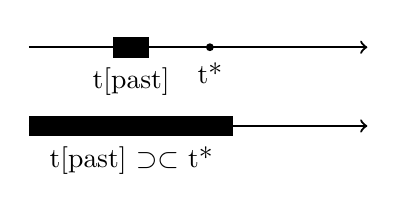
\begin{tikzpicture}[thick]
\tikzstyle{block} = [draw,minimum height=1pt,minimum width=12pt, fill=black]
\tikzstyle{dot} = [circle, fill=black,inner sep=1pt,minimum size=0pt]
\tikzstyle{block1} = [draw, minimum height=1pt, minimum width=73pt, fill=black]
% Pfeile übereinander
\coordinate (x1) at (0,0);
\coordinate (x2) at (0,1);
\draw[->] (-0.3,0) -- (4,0) coordinate[label = {}];
\draw[->] (-0.3,1) -- (4,1) coordinate[label = {}];
% tpast
\node (a) [block,label={below:t{[past]}}, right of=x2, node distance=1cm] {};
% t*
\node (b) [dot,label={below:t{*}}, right of =a, node distance=1cm] {};
% t[past]supsetsubset
\node (c) [block1, label={below:{t[past] $\supset\subset$ t*}}, right of =x1] {};
\end{tikzpicture}
\end{center}
       %%%
%\includegraphics[scale=0.4]{Bustamante_imperfect_perfect.pdf}
}

\citet[115]{Bustamante2013} implements this ``aspectual requirement on the past tense'' in the \ili{Spanish} mirative in terms of the set of syntactic features such that C asks for a i[past, unbounded] feature, where the [unbounded] feature is the
contribution of the imperfective aspect, following \citet{Pancheva2003} who defines [unbounded] as setting up the event time as a superset of the reference time ($\text{RT}\subseteq\text{ET}$). In contrast, [bounded], the feature of the perfective, is defined as setting up the event time as a subset of the reference time ($\text{ET}\subseteq\text{RT}$).
Given this constraint on the aspectual morphology of the participle, \citet[51]{Bustamante2013} assumes that aspect contributes its usual interpretation to the assertion.\footnote{\label{fn:34} \citet[51--52]{Bustamante2013} claims that the aspectual contribution of the imperfect is the imperfective aspect. Following \citet{Kratzer1998}, she assumes the latter to locate the reference time within the event time (RT\,$\subseteq$\,ET); see \REF{def:imperfect}:
\ea\label{def:imperfect}
\sib{imperfective} $ = \lambda P.\lambda t.\lambda w. \exists e [t \subseteq \tau(e) \wedge P(e)(w)=1]$.
\z}

%aspect has an impact on the mirative interpretation exerted through the assertion.

%Comparing the aspectual properties of the imperfect in the Peninsular \ili{Spanish} mirative and the pluperfect in the Andean \ili{Spanish} mirative, \cite[10--11]{Bustamante2013} concludes that the imperfective aspect of the former is associated with generic and habitual eventualities, whereas the pluperfect mirative is used for eventualities that are seen as culminated.\footnote{\cite[11,65--72]{Bustamante2013} argues further that this distinction is reflected by the nature of the surprise expressed by the two constructions, unlikelyhood vs. counter expectation respectively, thus arguing that also aspect contributes to the mirative meaning.}

%The speaker's beliefs should be relevant to the topic of the assertion. Therefore, the assertion should be sensitive to the distinction episodic-generic p. 14--15

Finally, \citet[14]{Bustamante2013} points out that the \ili{Spanish} mirative is not a direct expression of surprise in that the mirative operator does not encode surprise by itself. Instead, surprise is pragmatically derived from the clash between the recently discovered facts and what the past beliefs imply. This distinguishes the \ili{Spanish} mirative from exclamations and exclamatives which can express a wider range of speaker emotions. Being compatible with the expression of surprise, though, the mirative can be embedded under an exclamatory illocutionary operator (\textsc{exc}; defined in \citealt{Gutierrez-Rexach1996}), assuming the structure in \figref{fig:excl-mir}.

\begin{figure}[h]
%\includegraphics[scale=0.6]{EXC_CP_Bustamante.pdf}
 \begin{forest}
 for tree={s sep=1cm, inner sep=0, l=0}
  [Speech Act
   [\textsc{exc}]
   [CP
    [\qquad\qquad, roof]
   ]
  ]
 \end{forest}
\caption{Embedding CP under an exclamatory operator \citep[162]{Bustamante2013}}
\label{fig:excl-mir}
\end{figure}

%Bustamante p. 162: 36 speech act applied to CP where CP may be modified by an INOP or another evidential operator

As compared to the \ili{Spanish} mirative, the \ili{Bulgarian} admirative has not only modal, temporal, and aspectual, but also evidential properties that need to be accounted for. I therefore suggest that in addition to a modal base of past beliefs, the \ili{Bulgarian} admirative explicitly introduces an evidential component in terms of (i) the evidence acquisition time (EAT) that precedes (in inferential and reportative contexts) or coincides with (in direct evidence contexts) the speech time ($\text{EAT}\leq\text{ST}$) and (ii) the requirement that the speaker's belief base at discovery time entails the asserted proposition, i.e. the speaker has some evidence for the assertion prior to or at the time the assertion is made.\footnote{Idea (i) is adopted from \citeposst{Smirnova2011b} definition of the evidential modal operator \textsc{ev}.}
%\footnote{Alternatively, the admirative operator may introduce an additional proposition representing the evidence for the assertion that the speaker acquires at t'. The content of this proposition would be supplied by the context.}
Although \ili{Spanish} miratives do not have evidential morphology,
%, but they are felicitous in both direct and indirect evidential contexts.
the evidential meaning component of the \ili{Bulgarian} admirative fits naturally with the mirative semantics defined for the \ili{Spanish} construction: the belief clash the admirative expresses is caused by some evidence and the existence of such evidence is suggested by the admirative itself, not merely by context.\footnote{Note that similar to the \ili{Spanish} operator \textsc{m}\textsubscript{op}, the \ili{Bulgarian} admirative operator is covert, since its morphology is not unambiguous enough to trigger a mirative interpretation independently of context.} It also fits with \citeauthor{Bustamante2013}'s (2013: 57) observation that while the discovery time usually coincides with ST, there are cases where the discovery time precedes ST, like reporting news by means of miratives as well as miratives embedded under predicates like \textit{to turn out}. This accounts also for the \ili{Bulgarian} data discussed in \sectref{sec:BG-admirative}. Although the admirative operator employs the usual temporal precedence relation, the relation between EAT and ST is best captured in terms of an immediate precedence (the abut-relation $\supset \subset$), which accounts for \citeposst{Rett.Murray2013} recency requirement mentioned in \sectref{sec:decl}.

Similar to the \ili{Spanish} mirative, the mirative interpretation of the \ili{Bulgarian} admirative involves reference to a present eventuality, speaker commitment to the truth of $p$, and can be seen as the result of a displaced interpretation of the temporal feature of the past imperfect participle within the domain of the admirative operator \textsc{admir}. The operator introduces a modal base of past beliefs that implies a proposition contradicting the asserted proposition, and binds the temporal variable of the assertion in TP to ST.
The clash of old and new beliefs is caused by evidence for the asserted proposition.
The operator is defined in \REF{def:admir}, where $P$ is the modal base specified by the accessibility relation $R$ defined in \REF{def:R} above,
%w$_1$ is the actual world, t$_1$ is the speech time,
$t'$ is the EAT introduced by the admirative, and $Q$ represents the assertion.

\eanoraggedright\label{def:admir}
\textsc{admir} = $\lambda P \lambda Q \lambda t_1 \lambda w_1 \exists t' [ (t' \leq t_1 ) \wedge \allowbreak [ P(w_1)(t_1) \subseteq \lambda w \neg Q(w)(t_1)] \wedge \allowbreak Q(w_1)(t_1)] \allowbreak \wedge [\lambda w'[ w'$ is compatible with speaker's beliefs in $w_1$ at $t'] \allowbreak \subseteq Q(w_1)(t')]$
\z

\noindent When applied to the assertion, the operator \textsc{admir} yields the following interpretation of the admirative construction: admirative sentences are assertions based on evidence of some sort (reportative, inferential, direct) contrasted against the speaker beliefs that hold up to the speech time which may coincide with the discovery time or succeed it.
%This means that the speech time, rather than the discovery time, is the point up to which the past beliefs of the speaker hold. This may appear unjustified, since it is more natural to assume that the beliefs of the speaker get revised the moment the evidence is acquired, rather than the moment the speaker indicates that
The speaker's past beliefs entail a conclusion that clashes with the assertion, which triggers belief revision, while the actual current beliefs at $t'$ entail the assertion.
I further assume that, similar to the \ili{Spanish} mirative, the \ili{Bulgarian} admirative does not encode surprise itself, but the sense of surprise associated with it is rather a result of the clash between what the past beliefs imply and the recently acquired new belief. Its compatibility with the expression of surprise makes the exclamatory environment especially suitable for the admirative, which is accounted for by assuming a structure like the one presented in \figref{fig:excl-mir} for the \ili{Spanish} mirative.

In terms of the aspectual makeup of the participle and the reason why it is restricted to unbounded eventualities, similar assumptions can be made for the \ili{Bulgarian} admirative as for the \ili{Spanish} mirative. However, additional assumptions are needed for the distinction between \textsc{morphological aspect} related to the opposition imperfect : aorist and \textsc{situation} or \textsc{viewpoint aspect} related to the distinction between imperfective and perfective lexical forms in \ili{Bulgarian}. With \citet{Rivero.Slavkov2014} I distinguish between morphologically imperfect past participles like, e.g., \textit{pišel} and morphologically perfective (aorist) past participles like \textit{pisal}. In addition, I adopt their assumption that ``the morphological contrast between imperfect tense and aorist tense inflections (imperfect \textit{-še} vs. aorist \textit{-a}) systematically encodes imperfective vs. perfective viewpoints in the semantics'' \citep[235]{Rivero.Slavkov2014}. This applies to both indicative imperfects and aorists and their participles, where I assume the same semantics for the imperfective and perfective as in \citeauthor{Bustamante2013} (see fn. \ref{fn:34}). Consequently, \ili{Bulgarian} imperfect imperfective participles have the two features [past] and [unbounded], which is the required combination to feed the temporal argument of the modal base, as shown above. The ban on aorist and perfective forms in admirative sentences is explained by the introduction of the feature [bounded] by the aorist and perfective participles which always entails a past eventuality and disallows the displacement of the [past] feature.

A further reason why the \ili{Bulgarian} admirative construction is restricted to morpholgically imperfect and lexically imperfective participles seems to be related to the fact that a participle combining perfective aspect with imperfect tense like \textit{napišel} in \REF{ex:napisel} is restricted to specific, repetitive contexts.

\ea\label{ex:napisel}
\gll Vseki păt kogato napišel edno izrečenie, Petăr otival da puši.\\
every time when write.\textsc{ipf.pfv.ptcp} one sentence Petăr go.\textsc{ipf.ipfv.ptcp} \textsc{ptcl} smoke.\textsc{3sg.prs}\\
\glt `Each time Petăr wrote a sentence he went to smoke, it is said.'
\z

\noindent The use of perfective aorist participles seems in general less restricted; however, this combination can only be used in conclusives and renarratives (like the present perfect), as the aorist is banned in admiratives; see \REF{ex:napisala} and \REF{ex:napisala2}.

% % %     \largerpage[-1]

\eanoraggedright\label{ex:napisala} \textit{Context:} I see a picture of my good old friend Maria on a book in a window of a book shop and conclude that Maria has published a book. I say to myself:

\exi{}{\gll Maria \minsp{*(} e) napisala kniga! \\
Maria {} is write.\textsc{aor.pfv.ptcp} book\\
\glt `Maria has written a book!'}
\ex\label{ex:napisala2} \textit{Context:} Ivan tells me that Maria has written a book. I find this exciting and later tell Petăr:

\exi{}{\gll Ti ču li? Maria napisala kniga! \\
you hear.\textsc{aor.2sg} \textsc{q} Maria write.\textsc{aor.pfv.ptcp} book\\
\glt `Did you hear? Maria has written a book, they say!'}
\end{exe}

\noindent As a matter of fact, admiratives allow for the combination of secondary imperfective verbs and imperfect participle, as shown in \REF{ex:izmisljal}.

\eanoraggedright\label{ex:izmisljal} \textit{Context:} Ivan tells me that Maria has written a bestseller. Later, I meet Maria who denies that she has ever written a book. I suddenly realize that Ivan may have acquired a bad habit of making things up and exclaim

\exi{}{\gll Znači toj si izmisljal!\\
mean.\textsc{3sg.prs} he \textsc{refl} make.up.\textsc{ipf.pfv.ptcp}\\
\glt `So he is making up things!'}
\end{exe}

\noindent Here, the temporal interpretation is that of a present (habitual) eventuality, which however carries over to the past event of Ivan telling the speaker a lie. This shows that the interplay of morphological and viewpoint aspect in the case of the \ili{Bulgarian} admirative may be more complex than what has been assumed above. However, spelling out this contribution in detail is an issue that must be left to future work.
%with izmislil : znaci toj si go e izmislil! Conclusive under EXCL

\section{Summary and discussion}\label{sec:summary-disc}

In this paper, I provided an analysis of the \ili{Bulgarian} admirative in terms of a modal operator that captures the evidential, temporal, and aspectual properties of the construction.
In this section, I discuss some consequences and residual issues related to the analysis presented above.

First of all, assuming that the admirative indicates a clash of beliefs accounts for the sense of epistemic uncertainty observed in, e.g., \citet[510]{Smirnova2013} who argues that ``the evidential in direct contexts expresses commitment that is weaker than knowledge''.\footnote{See a similar claim in \citet[25]{Friedman1981} saying that \ili{Bulgarian} evidential forms in direct contexts express ``some state of ignorance or disbelief''.}

Second, in order to fully account for the place of the admirative in the evidential system, operators for the renarrative and the conclusive need to be defined that adequately capture their properties discussed in the previous sections:

\begin{itemize}
    \item Concerning the renarrative, such relevant properties are:

    \begin{itemize}
        \item It can be formed by both imperfect and aorist participles of both imperfective and perfective verbs, where imperfect participles in renarrative forms get either past or present interpretation depending on context.
        \item It does not commit the speaker (but possibly the reporter) to the proposition.
        \item It indicates that the evidence is acquired before the speech time \linebreak ($
        \text{EAT}<\text{ST}$).
        \item It can be embedded under an illocutionary exclamative operator with interpretations ranging from surprise or disbelief to a number of further emotive attitudes.
        \end{itemize}

    \item As for the forms of the conclusive:
%get only past interpretations,
    \begin{itemize}
        \item They exhibit both types of past participles and aspectual forms.
        \item They relate the assertion to the speaker's beliefs (thus involving a modal base).
        \item They indicate that the evidence is acquired before the speech time ($
        \text{EAT}<\text{ST}$).
        \item They are embeddable under an illocutionary exclamative operator.
        \end{itemize}
%concl also: no abut; internal and external evidence; it is modal: assertion related to beliefs of speaker

    \end{itemize}

In addition, appropriateness conditions need to be specified that govern the application of one or the other evidential operator.

%Alternatively: surprise in terms of conventional scalar implicature that p was less expected - \citet{Zanuttini.Portner2003}, but pragmatic appoaches to mirativity such as \citet{Rett.Murray2013} do not explain the morphological restrictions and the fake past interpretation - already mentioned
%Mention \citet{Ivanova-Sullivan2007}

%Like Izvorski, Smirnova analyses the \ili{Bulgarian} evidential in terms of an epistemic modal operator. In order to incorporate the direct evidential contexts into her analysis, however, she takes a different approach in which the meaning of the evidential construction is defined compositionally in terms of a tripartite, i.e., temporal, modal and evidential, semantic contribution.
%Unlike traditional grammarians (and simiarly to Izvorski), Smirnova distinguishes morphologically between present \textit{l}-participles, as in the evidential forms \textit{pi\v{s}e-l} (‘written’), \textit{svire-l} (`played'), glossed (\textsc{pres.ple}), and past \textit{l}-participles, as in the evidential forms \textit{pisa-l} (`written') or \textit{sviri-l} (`played'), glossed \textsc{past.ple} (cf. e.g. \citep[278--279]{Smirnova2011a}).

%According to Smirnova, the present/past tense marking of the participle stems encodes what she calls "evidential tense", arguing that the evidential stems do not encode aspectual difference but carry temporal information that she specifies in terms of a relation between some contextually salient reference time (RT in the neo-Reichenbachian framework of \citet{Klein1994}) and the time the speaker acquires the evidence (EAT, evidence acquisition time, originally introduced in \citet{Lee2011}).
%She argues further that the evidential tense of the participle stems, together with the (imperfective/perfective) verbal aspect, "jointly entail how the eventuality is located with respect to the EAT". Thus, past imperfective forms such as \textit{pisala} specify that the eventuality of writing is ongoing at RT (imperfective aspect: RT$\subseteq$ET, where $\subseteq$ is a relation of temporal inclusion) located in the past of EAT (past stem: RT$<$EAT, where $<$ is a precedence relation), from which it follows that the eventuality is in the past with respect to EAT, \citet[499--500]{Smirnova2011a}. %DOES SHE GIVE EXAMPLES WITH PAST PERFECTIVE forms? YES: exp. 38 p. 499 2011a
%A present evidential stem like \textit{pi\v{s}ela} signals on the other hand that the two times coincide (RT=EAT).
%In sum, Smirnova argues that \textsc{Ev} encodes the following complex information as part of its truth-conditional meaning:
%(i) external evidence (hearsay, direct evidence, inference from observation) as information source; (ii) universal modal force: the proposition is evaluated with respect to a modal base (the set of propositions believed to be true) of the speaker (in direct/inferential contexts) or reporter (in reportative contexts), and (iii) a temporal relation EAT$\leq$ST, where the correct relation is resolved when \textsc{Ev} interacts with sentence mood: EAT$<$ST when under DECL and EAT=ST when under EXCL.

%In addirion, a mechanism
%that would enable discourse participants to understand the temporal
%location of ET with respect to ST. In order to access this information,
%speakers need to know the relation between EAT and ST. this information is encoded in the meaning of the
%evidential operator. which is in point 3 above: EAT $\leq ST$

Third, allowing the temporal relation between discovery time and speech time to be one of either precedence or coincidence accounts for the fact that admiratives can be based not only on direct but also inferential and reportative evidence where the discovery time temporally precedes the speech time ($\text{EAT}<\text{ST}$). This is the case in \REF{ex:izmisljal} above. A further example illustrating this is \citeposst{Koev2017} deferred relalization example cited in \REF{ex:late-realization}, where the speaker ``has direct evidence for the described event but the realization that she does comes at a later time'' \citep[4]{Koev2017}:\footnote{\citeauthor{Koev2017}'s glosses are kept.}

\eanoraggedright\label{ex:late-realization}\textit{Context:} One of Nixon's aides vividly recalls walking into the Oval Office and seeing the President erase some tapes. She later learns about the Watergate scandal from the media and makes sense of what she had seen. When asked what happened on that day, she says:

\exi{}{\gll Kogato vljazo-x, Niksăn trie-še njakakv-i zapis-i. Toj zaličava-l ulik-i-te.\\
when enter-\textsc{past} Nixon erase-\textsc{past} some-\textsc{pl} tape-\textsc{pl}. he remove-\textsc{ev} clue-\textsc{pl-def}\\ \\
\glt ‘When I walked in, I saw Nixon erase some tapes. He was covering up the clues, as I learned later.’ \hfill \citep[4]{Koev2017}}
\end{exe}

\noindent \citet[4]{Koev2017} argues that this is not an example of mirativity, but a ``truly evidential interpretation'', since miratives are, according to him, conventionally accompanied by exclamative intonation and the speaker need not be surprised that Nixon was covering up the clues, as she may have heard about the Watergate scandal before uttering the sentence.
There are, however, some arguments in favor of treating such cases of late realization in terms of mirativity. As already pointed out, mirativity is not necessarily accompanied by exclamative intonation and involves (sudden) discovery or realization typically related to a clash of beliefs.
%Going back to \REF{ex:late-realization}, the speaker is not surprized over the fact that Nixon was covering up the clues, but over the discrepancy of what she believed to be an innocent tape-erasing and what she later realized was in fact covering up clues.
Besides, the direct evidence the speaker in \REF{ex:late-realization} has is that of Nixon erasing some tapes, rather than of Nixon covering up clues. It is therefore more plausible to assume that at the time of obtaining this direct evidence, the speaker did not have information about the Watergate scandal, since otherwise she would have realized (inferred) that the event of tape-erasing she had witnessed was in fact/at the same time an event of covering up clues, or that the tape-erasing was done with the aim of covering up clues.
%The additional knowledge she obtains leads to the sudded realization that the event she witnessed was not what she believed it to be at the time of acquiring the evidence.
The use of the zero-auxiliary form can thus be interpreted in terms of deferred realization and clash of old and new beliefs, which is the content of the admirative: the speaker's past beliefs entail the belief `Nixon was erasing some tapes' acquired through direct observation; upon acquiring information about the scandal, the speaker realizes that Nixon was not just erasing some tapes, but by doing this was actually covering up clues, which runs against what the speaker believed earlier.

The analysis of late realization cases like \REF{ex:late-realization} in terms of mirativity is also supported by typological evidence, see, e.g., \citet[441]{Aikhenvald2012} who discusses mirative statements that are based on visual evidence or inference and ``post-factum interpretation of the action judged by the results''.
%- exp. (2), as well as p. 460 exp. 32 and p. 468 deferred realization and 471!!
%"immediate/sudden evidence/realization"
The main argument that \citeauthor{Koev2017} uses to rule out a mirative interpretation is related to the fact that the discovery time in the example temporally precedes the speech time, which is incompatible with direct evidential sources. This temporal relation is, however, compatible with the meaning of the admirative defined in \REF{def:admir}, as well as with the clash of old and new beliefs based on some evidence that it encodes. Besides, it could be argued that the evidence leading to the mirative interpretation is not the directly observed event of tape-erasing, but the realization of the fact that the tape-erasing was in fact an act of covering up clues.

On the other hand, the eventuality referred to by the utterance is located in the past, not in the present, as was assumed for admirative sentences, which poses a problem for the analysis of \REF{ex:late-realization} in terms of mirativity.
%In order for the admirative operator to apply, a second past must be somehow present in TP, in addition to the displaced [past] feature of the imperfect participle, in order for the assertion to get past tense interpretation. This second past-feature must be somehow related to the late realization: what is surprizing is not the fact that Nixon was covering up clues but that the speaker didn't realize this fact given the knowledge that he had, namely the observation that Nixon was erasing tapes.
%Here, the speaker has direct evidence for the described event of Nixon covering up clues, but the realization that she does comes at a later time by means of inference based on what was observed and the additional information about the scandal she later acquires.
One possible solution would be to assume that the past interpretation follows from the precedence relation between the discovery time and the speech time ($\text{EAT}<\text{ST}$) and the fact that the contextually salient time that is relevant for the interpretation of the assertion is the time of the originally observed evidence, rather than ST ($\text{RT}=\text{EAT}$), which results in $\text{RT}<\text{ST}$ (${}=\text{past}$).
Interestingly, the form of the participle in \REF{ex:late-realization} is the same as in \REF{ex:izmisljal}: a combination of imperfect participle and secondary imperfective verbal aspect. Figuring out how exactly cases of deferred realization with this morphology fit the analysis presented here must be left to future work.

%So we have 2 EATs here: EAT1: e1 (=Nixon erases tapes), direct evidence, and EAT2 e2 (=Nixon is covering up clues), inference from e1 and additional knowledge on scandal. At EAT1 S believes q (Nixon erases tapes) and does not believe p(Nixon is covering up clues). At EAT2 S believes p and realizes that e1=e2, ergo S does not believe q anymore.

%observation does not lead to realization:


%(cf. also examples in Levin-Steinmann - a to bilo za dobro, tolkova i bilo pisano) and Bustamante on reports on belief change ! where EAT precedes ST

%cf also the pluperfect in Bust.

%This is another difference between the renarrative and the admirative: the renarrative does not require the reported evidence to immediately precede the speech time, whereas in the case of the admirative this has been pointed out as a crucial property (cf. Bustamante's abut-relation and section XX). But this is a different case: here the mirative is appropriate also in a context where the evidence is not just acquired.

Finally, a residual question that needs to be addressed in future work concerns the origin of the admirative. \citet{Nicolova2013} argues that the admirative originated from the perfect in its function to ascertain the existence of results from non-observed actions. This fits the crosslinguistic observation in \citet[73--74]{Bybee.Dahl1989} of indirect evidential uses licensed by the perfect due to its property of expressing past actions with present results: The indirect evidential uses can be viewed as extensions of ``known by its results'' to ``action known by inference/reports'' (see also \citet{Lau.Rooryck2017} who talk about knowledge of an event by indirect means). However, this path would immediately explain the emergence of the inferential and hearsay uses of the admirative out of the present perfect, but not the direct evidence uses. To shed more light on this issue, diachronic and typological data need to be thoroughly examined.

\section*{Abbreviations}
\begin{tabularx}{.5\textwidth}{@{}lQ}
\textsc{admir} & admirative operator\\
\textsc{aor} & aorist\\
\textsc{acc} & accusative\\
\textsc{def} & definite\\
\textsc{exc} & exclamative operator\\
\textsc{ev} & evidential (operator)\\
\textsc{imp} & imperative\\
\textsc{inf} & infinitive\\
\textsc{ipf} & imperfect \\
\textsc{ipfv} & imperfective aspect\\
\end{tabularx}\begin{tabularx}{.5\textwidth}{lQ@{}}
\textsc{m}\textsubscript{op} & mirative operator \\
\textsc{neg} & negation\\
\textsc{pfv} & perfective aspect\\
\textsc{pl} & plural\\
\textsc{prs} & present tense\\
\textsc{ptcl} & particle\\
\textsc{ptcp} & participle\\
\textsc{q} & question particle\\
\textsc{refl} & reflexive pronoun\\
\textsc{sg} & singular\\
\end{tabularx}

\section*{Acknowledgements}
I would like to thank the participants of the \textit{13th European Conference on
Formal Description of \ili{Slavic} Languages} in Göttingen for discussing an earlier version of this work, as well as Torgrim Solstad and two anonymous reviewers for valuable comments and suggestions. A special thanks goes to my informants for their native speaker judgements.

{\sloppy\printbibliography[heading=subbibliography,notkeyword=this]}

\end{document}
